%%「論文」,「レター」,「レター(C分冊)」,「技術研究報告」などのテンプレート
%% 1. 「論文」
%% v1.6 [2009/11/03]
\documentclass{ieicej}
%\documentclass[invited]{ieicej} % 招待論文
%\documentclass[comment]{ieicej} % 解説論文
\usepackage{graphicx}
\usepackage{float}
\usepackage{latexsym}
\usepackage[fleqn]{amsmath}
\usepackage[psamsfonts]{amssymb}

\setlength\intextsep{10pt}
\setlength\textfloatsep{0pt}

\setcounter{page}{1}

\field{A}
\jtitle{MultiPath TCP適用時のデータセンターネットワークでのフローサイズが与える影響に関する一考察}
\etitle{A study of the effect of the size of data flows in the data center network with MultiPath TCP}
\authorlist{%
 \authorentry{藤居 翔吾}{Shogo Fujii}{Tokyo}% <= 記述しないとエラーになります
 \authorentry{関谷 勇司}{Yuji Sekiya}{Tokyo}
 \authorentry{田崎 創}{Hajime Tazaki}{Tokyo}
 %\authorentry{和文著者名}{英文著者名}{所属ラベル}
 %\authorentry[メールアドレス]{和文著者名}{英文著者名}{所属ラベル}
 %\authorentry{和文著者名}{英文著者名}{所属ラベル}[現在の所属ラベル]
}
\affiliate[Tokyo]{東京大学大学院工学系研究科, 文京区}{Graduate School of Engineering,
Tokyo University, 7-3-1, Hongo, Bunkyo-ku, Tokyo, 113-0033, Japan}
%\affiliate[所属ラベル]{和文所属}{英文所属}
%\paffiliate[]{}
%\paffiliate[現在の所属ラベル]{和文所属}

\begin{document}
\begin{abstract}
%和文あらまし 500字以内
データセンター内で運用されるサーバ台数の増加に伴い, それらを効率良く利用するためのネットワークトポロジーが研究されてきた.
近年では, Multipath TCPを用いて, さらなるネットワークリソースの有効活用を目指す取り組みが行われている.
さらに, 大規模データを効率的に分散処理させるソフトウェアとしてHadoop, MapReduce等の分散処理技術に関する研究により,
大規模データを大規模サーバで処理するデータセンターにおいては, それらの分散処理技術が必要不可欠である.
近年の分散処理技術では, 計算処理とデータ格納の役目を担う「処理ノード」と,
個々の処理ノードでの進捗状況やデータの書くのを管理する「管理ノード」の二種類から構成されている.
すなわち, 管理ノードから発行されるqueryを処理ノードが実行する, query-workerモデルであり,
フローサイズの小さいqueryトラフィックが発生する.
Multipath TCPは複数の経路を同時に利用し, ネットワーク資源の有効活用を実現するが,
フローサイズの小さいトラフィックに関しては,
TCPよりも処理の完結に時間がかかり, その有用性に問題を抱えていると言える.
そこで本論文では、Multipath TCPを用いたデータセンターネットワークの有用性を検証し, Multipath
TCPのショートフローに対する問題点を考察する.
\end{abstract}
\begin{keyword}
%和文キーワード 4〜5語
マルチパスTCP, MultiPath TCP, Short Flow, フロー完結時間, FatTree Topology
\end{keyword}
\maketitle

\section{まえがき}
\label{sec:intro}

近年,




-まえがきstart-\\
\\
\\
\\
\\
\\
\\
\\
\\
\\
\\
\\
\\
\\
\\
\\
\\
\\
\\
\\
\\
\\
\\
\\
\\
\\
\\
\\
\\
\\
\\
\\
\\
-まえがきend-

\section{関連研究}
本章では, これまでに報告されているマルチパス利用によるフロー完結時間短縮か技術について簡潔に述べ, その優位性や問題点を示す.
\begin{figure}[h]
    \begin{center}
    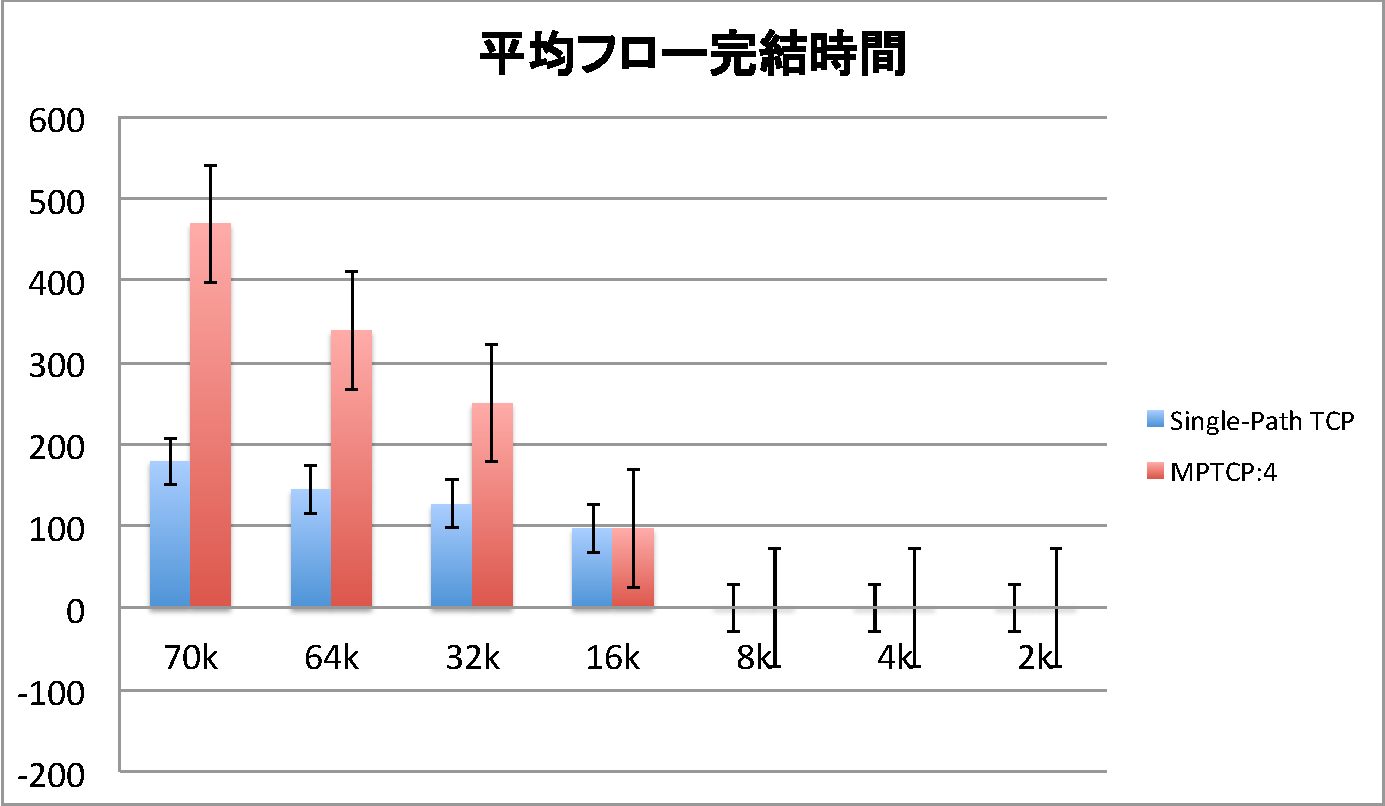
\includegraphics[width=150pt, bb=20 20 592 504]{./img/test.pdf}
    \caption{図の説明}
    \label{fig:one}
    \end{center}
\end{figure}

2010年にAlizadehらによって, データセンターネットワーク特有のトラフィックパターンに特化して, パラメータを決定するアルゴリズムが提案された.
データセンタートラフィックの引き起こす問題点として, Queueの生成によるレイテンシ, 大量のQueueの送信によるパケットロス,
スイッチのバッファに掛かる負荷, があり, Queueの蓄積を制御するためのしきい値をアルゴリズムから設定することで, これらの問題を解決し,
99.9パーセンタイルのQueueの伝送時間を短縮することを可能にした.
しかし, 大規模計算資源を想定したトポロジーにおける検証がされておらず, また, 各ネットワークデバイスに細かなチューニングを必要とするため,
大規模データセンターにおいては運用面での問題がある.

2011年にCostinらによって, Multipath TCPを用いたデータセンターネットワークモデルが提案された.
近年の大規模計算資源を有効活用するために提案されたネットワークトポロジーでは,
高性能なデバイスや特殊なデバイスを必要とせず, 汎用デバイスのみを用いてホスト同士の通信の際に経路が複数用意されている.
これまで複数の経路の内一つを選択し, 余分な経路をセカンダリ経路として, 耐障害性を持たせていたのに対し, 提案されたデータセンターモデルでは,
Multipath TCPを用い複数経路を同時に利用する事で, 耐障害性を保ちながら, 帯域を最大限利用する事を可能にした.
実際, 様々なトポロジーにMultipath TCPを適用することで, 従来のTCPよりも高いスループットが出せることを示した.
しかし, サイズの小さいフロー(<70KB)フロー完結時間に着目すると, TCPよりも時間がかかるという問題点があった.

2012年にZarsらによって, クロスレイヤーでトラフィックを監視し, しきい値を決定することによるフロー完結時間の短縮化技術を提案した.
サイズの異なるフローが混在するネットワークにおいては, サイズが小さいフローが, サイズの大きいフローに圧迫され, 伝送遅延が大きくなる問題があった.
そこで, データリンク層からアプリケーション層までの各層が, 相互にトラフィックを監視する機能をスイッチに実装し, 優先度をつけたり,
バッファサイズを調整することで, フロー完結時間の悪化を抑えることを可能にした.
しかし, 実験ではClick\cite{}を用いて, 特殊な実装を行っており, 汎用スイッチでクロスレイヤーの監視をすることはできない.

以上で述べたことをまとめると, 近年のデータセンターネットワークに対して, 以下のような要求が考えられる.
\begin{itemize}
  \item 大規模計算機を有効活用するトポロジーの利用
  \item 分散処理の際に発生する大量のサイズの小さいフローの送信時間の短縮
  \item 特殊な実装, デバイスを用いず, シームレスな運用の実現
\end{itemize}

\section{MultiPath TCP}
MultiPath TCPは, シングルパスを用いてデータ転送するTCPを拡張し, 複数のインタフェース,
あるいはポートを用いてデータ転送をするプロトコルである[\ref{mptcp}].
Multipath TCPは, ホスト同士がコネクションを確立する際にネゴシエーションが行われ, 互いにMultipath TCPを扱えるかどうかの確認を行う.
クライアントが複数のIPアドレスを持っていた場合, 新たにサブフローのコネクションが確立される.
追加されたサブフローは, クライアントの持つインターフェースが1つの場合, 最初のサブフローと同じペアーのIPアドレスで異なる送受信ポートを用いる.
その際, ルーティングに関しては, Equal Cost Multi Path(ECMP)により用いる
サブフローの分だけルーティングを行う.
インターフェースを複数持つ場合には, 異なるIPアドレスのペアを用いて, 通信を行う.
ルーティングに関しては, 複数対の宛先IPアドレス, 送信元アドレスを見て, ルーティングされる.

サブフローが確立するとすぐに, TCPスタックによりデータを転送する.
クライアントがデータを受けると, TCPの順序制御により, 元のデータを正しく組み立てられる.
このように, アプリケーション層より下のレイヤーのみで, データ転送を行うため, アプリケーション側がTCPの代わりにMultipath
TCPが使われた事を意識する事なく, データ転送ができる.

Multipath TCPでは, 各々のサブフローが,シークエンス領域を持ち, それぞれのサブリンクの状態に合わせて輻輳制御をする[\ref{}].
また, 輻輳制御に関しては, TCPと同様にAIMD(additive-increase and
multiplicative-decrease)による輻輳制御がサブフロー単位で行われる.
下記にAIMDアルゴリズムを示す.

\begin{itemize}
\item サブフロー $r$において,
1ACKごとにウィンドウサイズ$\omega_{r}$をmin$(\frac{a}{\omega_{total}},
\frac{1}{\omega_r})$増加させる.
\item サブフロー $r$において, パケットロス時にウィンドウサイズ$\omega_r$を$\frac{\omega_r}{2}$へ減少させる.
\end{itemize}
ここで, $\omega_{total}$は全てのサブフローのウィンドウサイズの総和, $a$は送信速度の増加量を示すパラメータで,
[\ref{}]にて定義される.

Multipath TCPでの輻輳制御において, 二つの性質が有る.
一つは, 大きいウィンドウを持つサブフローはより速くウィンドウサイズを増加できるという事である.
これにより, 混雑したサブリンクにおいては, ウィンドウサイズが抑えられ, ロードバランスができる.
二つ目は, もし全てのサブフローが同じボトルネックを抱えていたとき, パラメータ$a$を適用する事によって,
TCPフローの公平に帯域を利用できるという事である.
しかし, もし複数のサブフローがそれぞれ混雑のないサブリンクを利用する場合, いずれかのコネクションが帯域を占有する可能性がある.


\section{FatTreeトポロジーとMPTCPによるデータセンターモデル}
この章では, データセンターを構成する要素について述べる.
\subsection{トポロジー}
\label{subsec:topology}
従来のデータセンターモデルでは, hostがtop-of-rackスイッチにつながり,
これらのスイッチがaggregationスイッチに集約され,
またaggregationスイッチがcoreスイッチに接続するといったように, 階層的にトポロジーを形成していた.
このような階層構造を持つトポロジーは, トラフィックの大部分がデータセンターの外から入ってくる, あるいは出て行くような場合, 有効であった.
しかし, データセンター内で生じるトラフィックが大半を占める場合, 帯域の割当が適切でなくなる.
このような, ローカル環境でのトラフィックが主であれば, 階層型のトポロジーはボトルネックを引き起こす可能性がある.
近年の研究では, トラフィックがローカルに集中した時の問題を, 物理的なアプローチとして, トポロジーを工夫する事で解消しようとしている.

VL2, FatTreeトポロジーでは, coreスイッチを複数用いる事で, 物理パスの最大帯域を供給する.
FatTreeトポロジーでは, 比較的狭い帯域のパスを多用するのに対し, VL2トポロジーでは, 広い帯域のパスを少量用いる, といった違いがある.
また, BCubeは階層構造ではなく, 超立方体の形をとり, ホストがパケットリレーに参加するようなトポロジーである.

これら3つのトポロジーを用いる事で, データセンター内のトラフィックに対し, 帯域を十分に使う事ができる.
しかしこのような密な配置により, 複数の経路が形成され, ルーティングをどのように決定すべきか, という問題も生じる事となる.

\subsection{ネットワーク資源の有効活用}
近年提案されたトポロジーは, 密度の高い相互接続性を持ち, ホスト同士の通信の際に, 複数の経路を形成をしている.
例えば, 図~では\ldots\ldots
しかし, ホスト自身はどの毛糸が最も混雑していないのかを認識できないため, ルーティングシステムにより, 複数の経路を有効活用する必要がある.
最も単純な方法は, ECMPルーティングにより, 通信可能な経路の中からランダムに選び, 経路を選択するというものである.


\section{データセンターにおけるトラフィックシナリオ}
本性では, データセンターにおけるトラフィックの特性について, 考察を行う.

近年のデータセンターが有するサーバ数は, 扱うデータ量の増加に従って, 増加の一途を辿っており, 大量の計算機資源を有効活用するために,
アプリケーションとして分散コンピューティングフレームワークを用いる.
Hadoop, Mapreduce等が現在フレームワーク使われており, 一般的に図\ref{}に示すようにpartition/aggregate構造をとる.
このような構造は, \ref{sec:intro}章で示したデータセンタートラフィックの性質から, \ref{subsec:topology}節で述べた,
近年提案されたトポロジーを用いる事が多い.
より具体的な応用例では, Webサーチ, SNSのリコメンド機能など, リアルタイムにレスポンスを返すようなシステムで用いられ,
多数の処理ノードと, 分散処理の制御をする管理ノードの二つのノードから構成されている.
具体的には管理ノードから, クエリーが発行され, 分散処理がクエリーを受け取り, 処理を行う, クエリーレスポンス
モデルに従っている.
クエリーレスポンスモデルである以上, そのトラフィックパターンが  (1){\it Query traffic}, (2){\it Short message
traffic}, (3){\it Backgroung traffic}の3つに分類される.

{\bf Query traffic. }Query trafficとは, 大規模計算処理を分割して並列処理する際に,
aggregatorノードから処理ノードへ具体的な処理を割り当てるためのトラフィックである.
Query trafficの特徴は, 非常に小さいフローサイズ(2KB$\sim$20KB)で、処理全体のレイテンシに非常に強く影響を及ぼす事である.
また分散処理システムの構成上, Query trafficは短時間に大量のフローを生成する.
図\ref{}に, Query trafficの生成時間間隔の分布を示す\cite{dctcp}.
Query trafficにおける, フローサイズはほとんど一定で1.6KB$\sim$2KBである事が多い.
また, ミリ秒単位でQueryが生成される, バースト性を持つ.

{\bf Short message traffic. } Short message trafficとは,
処理ノードの動作を制御するためのトラフィックである.
Short message trafficの特徴は, フローサイズは50KB$\sim$1MBで, Query
trafficと同様に処理全体のレイテンシに影響を及ぼすという事である.
しかし, Querry trafficほどのフロー数は生成されず, 生成時間感覚も秒単位である.

{\bf Backgroung traffic. }Backgroung trafficは, Queryに対するレスポンスの精度を高める,
核処理ノードへの更新データのためのトラフィックである.
Backgroung trafficの特徴は,フローサイズが1MB$\sim$50MBと大きいことにある.
さらに, その生成時間間隔は大きい.
また, Backgroung trafficでの更新データは, 処理精度の向上に寄与するが, 処理に必須ではないので,
それ自身のレイテンシが処理全体のレイテンシにはつながらない.
図\ref{}にデータセンタートラフィックにおけるフローサイズの分布を示す.
この分布から, 大半のフローサイズは小さいが, 全体の通信量の大部分がBackgroung trafficによるものだという事が分かる.
そのため, Backgroung trafficが物理パスの帯域を圧迫する傾向がある.

つまり, データセンターネットワークには, スループット依存なBackgroung traffic, 遅延依存な小さなフローShort message
traffic, バースト性を持つQuery trafficが混在している.


\section{ShortFlow評価と考察}

\subsection{Query traffic}

\subsection{Short message traffic}

\subsection{Backgroung traffic}

\subsection{Multipath TCP v.s. TCP}

aaaaaaaaaaaa


-ShortFlow評価と考察start--\\
\\
\\
\\
\\
\\
\\
\\
\\
\\
\\
\\
\\
\\
\\
\\
\\
\\
\\
\\
\\
\\
\\
\\
\\
\\
\\
\\
\\
\\
\\
\\
\\
\\
\\
\\
\\
\\
\\
\\
\\
\\
\\
\\
\\
\\
\\
\\
\\
\\
\\
\\
\\
\\
\\
\\
\\
\\
\\
\\
\\
\\
\\
\\
\\
\\
\\
\\
\\
\\
\\
\\
\\
\\
\\
\\
\\
\\
\\
\\
\\
\\
\\
\\
\\
\\
\\
\\
\\
\\
\\
\\
\\
\\
\\
\\
\\
\\
\\
\\
\\
\\
\\
\\
\\
\\
\\
\\
\\
\\
\\
\\
\\
\\
\\
\\
\\
\\
\\
\\
\\
\\
\\
\\
\\
\\
\\
\\
\\
\\
\\
\\
\\
\\
\\
\\
\\
\\
\\
\\
\\
\\
\\
\\
\\
\\
\\
\\
\\
\\
\\
\\
\\
\\
\\
\\
\\
\\
\\
\\
\\
\\
\\
\\
\\
\\
\\
\\
\\
\\
\\
\\
\\
\\
\\
\\
\\
\\
\\
\\
\\
\\
\\
\\
\\
\\
\\
\\
\\
\\
\\
\\
\\
\\
\\
\\
\\
\\
\\
\\
\\
\\
\\
\\
\\
\\
\\
\\
\\
\\
\\
\\
\\
\\
\\
-ShortFlow評価と考察end--

\section{あとがき}
-あとがき--\\
\\
\\
\\
\\
\\
\\
\\
\\
\\
-あとがきend--


\ack %% 謝辞
\\
-謝辞start--\\
\\
\\
\\
\\
\\
\\
\\
\\
\\
-謝辞end--
%\bibliographystyle{sieicej}
%\bibliography{myrefs}
\begin{thebibliography}{99}% 文献数が10未満の時 {9}
\bibitem{dctcp}{Alizadeh, Mohammad, et al. "Data center tcp (dctcp)." ACM
SIGCOMM Computer Communication Review 40.4 (2010): 63-74.}
\bibitem{improving}{Raiciu, Costin, et al. "Improving datacenter performance and
robustness with multipath TCP." ACM SIGCOMM Computer Communication Review. Vol. 41. No. 4. ACM, 2011.}
\bibitem{detail}{Zats, David, et al. "DeTail: Reducing the flow completion time
tail in datacenter networks." ACM SIGCOMM Computer Communication Review 42.4 (2012): 139-150.}


\end{thebibliography}

\begin{biography}
\profile{s}{藤居 翔吾}{平25 立命館大・工。電気電子卒. 同年東京大学大学院修士課程入学.
MPTCPを利用したデータセンターネットワーク等の研究に従事.
}
\profile{m}{関谷 勇司}{}
\profile{m}{田崎 創}{}
%\profile{会員種別}{名前}{紹介文}% 顔写真あり
%\profile*{会員種別}{名前}{紹介文}% 顔写真なし
\end{biography}

\end{document}